%%%%%%%%%%%%%%%%%%%%%%%%%%%%%%%%%%%%
% This is the template for CS7290 lecture notes which is based on ISCA
% 2017 submission.
% The cls file is a modified from  'sig-alternate.cls'
%%%%%%%%%%%%%%%%%%%%%%%%%%%%%%%%%%%%

\documentclass{sig-alternate}  
%\documentclass[10pt,onecolumn,notitle]{article}
%\documentclss{alternate}
\usepackage{mathptmx} % This is Times font

\makeatletter
\newcommand\resetstackedplots{
\makeatletter
\pgfplots@stacked@isfirstplottrue
\makeatother
}
\makeatother

\newcommand{\ignore}[1]{}
\usepackage{fancyhdr}
\usepackage{float}
\usepackage{tabularx}
\usepackage[normalem]{ulem}
\usepackage[hyphens]{url}
\usepackage{hyperref}
\usepackage{pgfplots}

%%%%%%%%%%%%%%%%%%%%%%%%%%%%%%%%%%%%


\fancypagestyle{firstpage}{
  \fancyhf{}
\setlength{\headheight}{50pt}
\renewcommand{\headrulewidth}{0pt}
  \fancyhead[C]{\normalsize{CS7290
      }}
  \pagenumbering{arabic}
}

%%%%%%%%%%%---SETME-----%%%%%%%%%%%%%
\title{CS6250 Fall 2017 
Profiling and Benchmarking Computational Offloading}
\author{F. Lotfi, R. Elliott Childre, T. Nguyen, S. Parab, A. Nagarajan  }
%%%%%%%%%%%%%%%%%%%%%%%%%%%%%%%%%%%%

\begin{document}
\maketitle
%\thispagestyle{firstpage}
%\pagestyle{plain}
%\date{\today}


\section{Abstract}
Mobile devices are ubiquitous and resource constrained.
However, users need an exceptional experience despite these constraints. To provide such an experience, we are looking to exploit the plentiful resources available in the cloud.This project hopes to solve this problem with a remote processing strategy known as cloud offloading. Many benchmarks were made that take pictures of a scene but allow an offsite server to do the image processing and then send the resulting image back to the device on which the images were captured.
The essence of this project is to strategize offloading for different applications to enhance user experience.

\section{Introduction}
Today everyone has a mobile device but these devices remain computationally constrained compared to laptops, desktops, servers, and super computers. Other limitations include battery, heat, memory, and threading limiting the potential for code optimization on device with current general purpose CPUs. Despite all of this users still demand and exceptional experience when using a mobile application. Increasing the applications that consume most of users time are photo and video manipulation apps like Snapchat and Instagram. The future likely holds more applications in the computer vision, graphics, and augmented reality space. Our solution to these pressing constraints on what can be done with on device resources and what is expected to be done is to look towards the cloud as computational accelerator. In this paper we present a benchmarking application we built to analyze which problem sets are best to be offloaded and what optimization techniques we can use to improve speed and bandwidth.
\section{Motivation}
Computational offloading is a broad problem  where depending on the goal you want to optimize for will result in different outcomes. Much of the focus in the literature today seeks to find answers for performance improvements, extending battery life, optimizing for Heat and power constraints (typically classified under the dark silicon problem), computational partitioning where you divide computation between the device and the cloud, and much more. We itemize the interesting areas of research below. 
\begin{itemize}
\item \textit{Performance}:
This is where much of the research we found interesting for our project lies. Essentially here we identify Where we can improve efficiency by offloading suitable algorithms to the cloud. We will do a literature review on this area in the background section of this paper.
\item \textit{Battery Life}:
Offloading might help us save battery on the mobile system. For an application like ours we would expect the screen and camera to be constantly running which we could treat as constant power draw. experimentation could be cpu utilization vs wifi  or modem power draw. Experimentation could further be done around distance from a cell tower or wifi access point as a way of varying any heuristic we derive for determining whether or not to offload. \cite{wifiBattery}
\item \textit{Computation Partitioning}:
 It is possible to partition an application to use both the cloud and local resources simultaneously.\cite{partitioning}
\item \textit{Dark Silicon}:
Most of the research around Dark silicon in mobile has been focused around coming up with new architectures like ARM big.LITTLE and the experimental GreenDroid. These are all solutions to try and overcome \textit{Dennard scaling} which states that as as transistors get smaller their energy density stays constant since voltage and current in the transistor scale downward as well. \cite{darkSilicon} GreenDroid is particularly interesting because they are creating an on-chip network router as a way of distributing processing across the die to minimize heat by utilizing as much surface area as possible. \cite{greenDroid}
Given they are already using distributive computing concepts to solve this problem it would not be too far fetch to think that if current chip design improvements fail to fully address this area, off device computation could be a path forward.
\item \textit{Server Availability}:
This topic attempts to address the question can you offload if your server is unreliable? If the cloud might not always be available for offloading can we gather a metric for the quality of the network? How much do we consider qualitative metrics like diminishing user experience?
\item \textit{Decision Overhead}:
There is an an overhead that needs to be consider when we periodically tests the network quality and makes dynamic decisions for offloading. The iPerf network profiling processing periods would routinely be one of our most high profile threading events in our Traceview dumps. These were done asynchronously so it did not show up in performance metrics but could have implications for some of the other goals to consider for this research topic like partitioning, and battery life. 

\end{itemize}
Lack of a budget for this project made battery life and power experimentation impossible as all of our testing were done on emulated android devices. We chose to focus instead on performance optimization and simulate 3G, 4G, and Wifi networks. The Server Availability and Decision overhead head questions required us to first build out a platform before we could make any progress on addressing these questions, so for scoping we do not address them in this paper. We should note that the literature around using computational offloading to solve the dark silicon problem is slim to none and could be an interesting focus of research. Since we will be focusing on performance we will try to constrain the problem sets we will try to improve to:
\begin{itemize}
    \item Image/Video processing applications
    \item Augmented Reality (AR) applications
\end{itemize}
\section{Background}
The basic idea of Computational offloading as laid out by \textit{Shi and Ammar COSMOS (Computation Offloading as a Service for Mobile Devices)} is to have a client component and a server component that can run the same code.\cite{cosmos} The client component needs to perform 3 basics functions. First, monitor and predict network performance.  Second, track execution requirements Third, choose some portion of code to execute remotely that can reduce computation time. Our implementation and paper will deviate from COSMOS in a few significant ways, for one we have no hardware or budget for on demand VM allocation. Or performance improvements will be limited to that of a single laptop server. Second, our platform is a benchmark suite similar to something like spec2000, So we want to answer the question of what types of problems are good to offload and what are not. COSMOS on the other hand is better suited for problems where you know what you want to offload. COSMOS also had a metric of cost it wanted to optimize for. This is a requirement we are ignoring for this paper, and is not as relevant for us as we do not lease computation time for our experiments.

Another research paper, CloneCloud \cite{clonecloud} by Chun and Ihm focuses on dynamically offloading only a part of the execution from the mobile devices to the cloud. CloneCloud was far more focused on taking any application and running it through a static analyzer to determine what improvements could be done for offloading. Our paper will try to pick a more constrained problem set to work with. Our paper will focuses on the offloading experimentation around image processing applications. We chose to focus only on the image processing applications.

\subsection{Decision Engine}
The COSMOS system achieves high performance offloading at a low cost by sharing cloud resources among the mobile devices. An optimization algorithm was proposed by the authors to determine the cloud resource management, the decision to offload and the task allocation, based on the assumption that the cloud can simultaneously run N virtual machine instances. \cite{cosmos}

The maximum speedup of using the COSMOS system against the local execution can be computed by solving the optimization algorithm.

\begin{figure}[H]
\begin{tabular}{ | m{5em} | m{5cm}| } 
\hline
K & \tiny Total computation tasks \\
\hline
M$_{i}$    & \tiny The type of the i$^{th}$ VM instance \\
\hline
T$_{i}$    & \tiny The leasing periods of  the i$^{th}$ VM instance \\
\hline
$\psi$(M,T)    & \tiny The pricing function for leasing a VM instance \\
\hline
O$_{k}$  & \tiny The k$^{th}$ computation task \\
\hline
I(i,k)   & \tiny The indicator function for offloading task O$_{k}$ to VM i   \\
\hline
I$_{l}$(k) & \tiny The indicator function for executing task O$_{k}$ locally  \\
\hline
L(O$_{k}$) & \tiny The local execution time of the task  O$_{k}$\\
\hline
R$_{i}$ (O$_{k}$) & \tiny The response time of offloading the task O$_{k}$ to VM i  \\ 
\hline
\end{tabular}
\begin{equation} 
 Max  \space \sum_{k = 1}^{K} \frac{L({O_{k}})}{\min_{ \frac{L({O_{k}})}{I_l(k)}, \frac{R_i({O_{k}})}{I(i,k)} |\forall_{i}}}
\end{equation}
\begin{equation}
  s.t. \space I_{t}(k) +\sum_{t = 1}^{N} I(i,k) = 1
\end{equation}

\caption{The COSMOS Optimization Algorithm.}
\end{figure}

In the COSMOS decision engine, to decide whether to offload or not depends on setting the Il(k) to 0 or 1. This is a challenge because of various network connectivity, program execution and resource contention issues. These uncertainties have to be dealt with for proper utilization of cloud resources and optimized speedup. \cite{cosmos}

For our uses we can drop variables T$_{i}$ and $\psi$(M,T) because cost is not a concern of this paper. Further we  will be redefining L(O$_{k}$) as T$_{computation\_device}$ and R$_{i}$ (O$_{k}$) as T$_{total\_server}$. We will further simplify our algorithm from being the sum of all compute tasks to each individual task as our heuristic will be highly specialized for the effect we want to optimize. For example the indicator for grayscale would likely be I$_{l}$(k) > .95 while one for something like Face swap would take more network health into consideration and thus I(i,k)  would be larger. More on this in \textit{Simplified Dynamic Offloading Decision Engine} section.

\section{Design}
\subsection{Objective}
Create a video editor  that allows different effects to be applied to the video, such as gray scale, blurring, negative, Face Swap, etc. The video should be captured directly from the camera. The editor should also have a well usable UI to apply any effects or editing features. The UI should consider best practices for an application  that targets phone or tablet form-factors. Finally, the application is expected to have good programmatic design and  well-documented function or method calls to allow for reproducibility of results by  an impartial red team.

\subsection{Core Android (Anchored Code)}
\begin{figure}[H]
\noindent 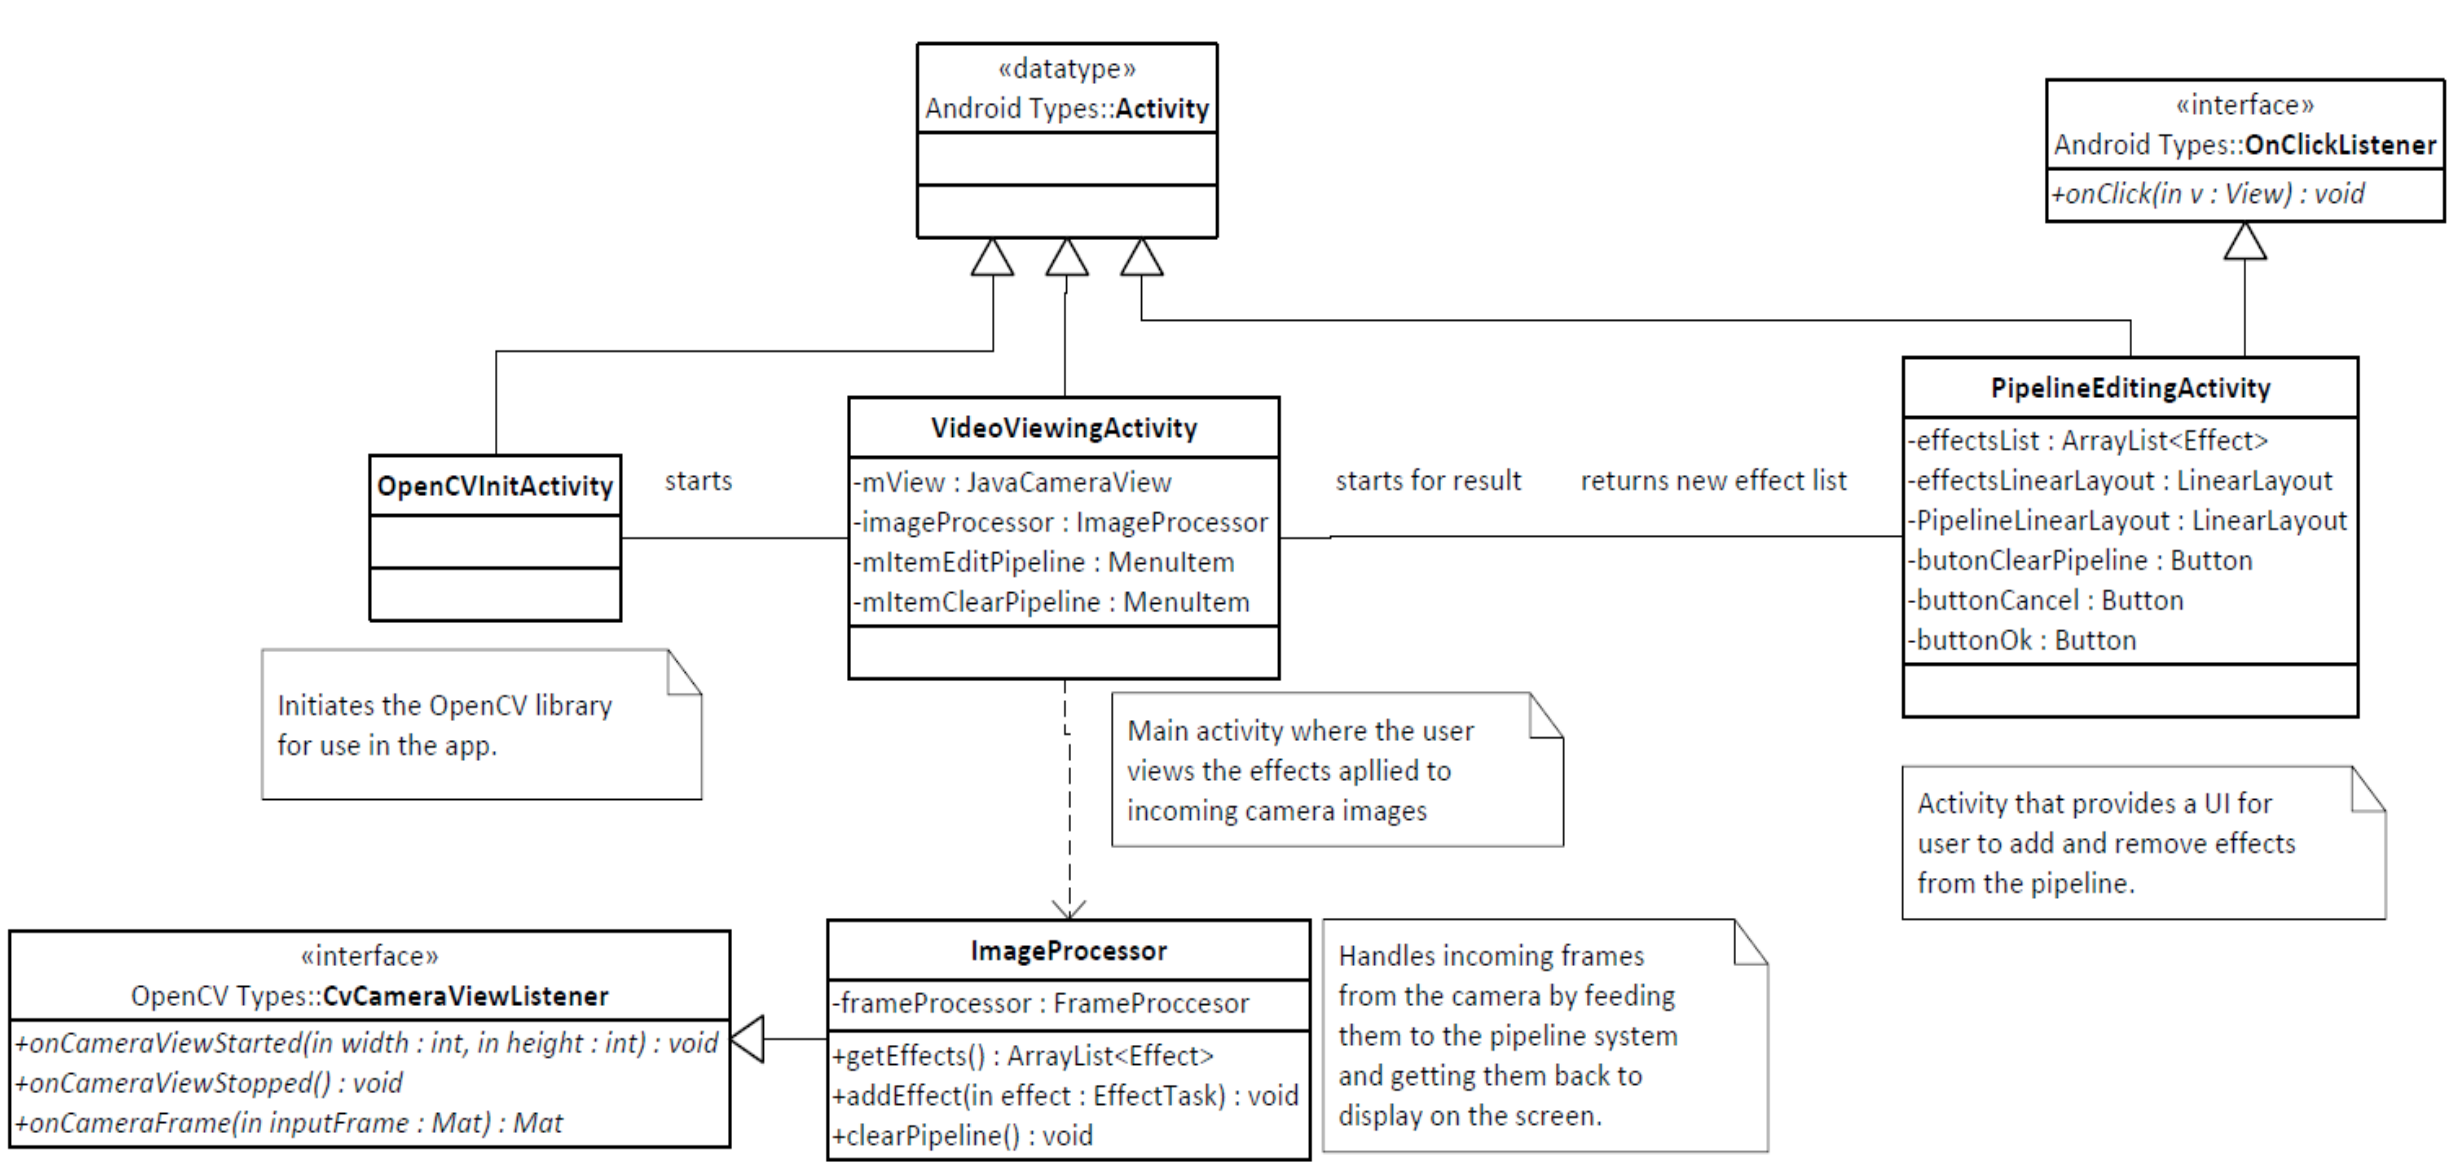
\includegraphics[scale=.2]{coreUML.png}
\caption{overview of the Android specific code.}
\end{figure}
Design patterns make up a big part of enabling whether or not an application can be offloaded. We took best practices from \textit{Refactoring Android Java Code for On-Demand Computation Offloading}. The most important way that we enable this is through pipelineing our effects. We need to be able to categorize our codebase into \textit{Anchored} and \textit{Moveable} class. Effects have no dependency on Android code and the camera image fetches are abstracted to the beginning of the pipeline and have no barring on later section of the pipeline. \cite{AndroidRefactor}

\begin{figure}[H]
\noindent 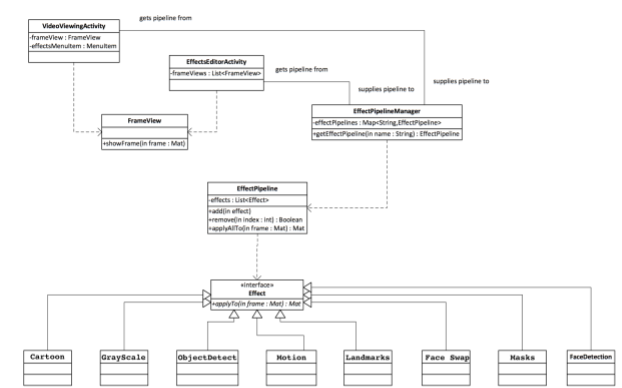
\includegraphics[scale=.3]{ApplicationOverview.png}
\caption{Application overview.}
\end{figure}
\begin{figure}[H]
\noindent 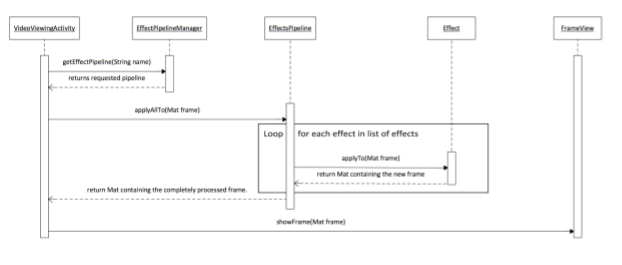
\includegraphics[scale=.3]{FramePipline.png}
\caption{Displaying a Frame}
\end{figure}

\subsection{Effects (Moveable Code)}
\begin{figure}[H]
\noindent 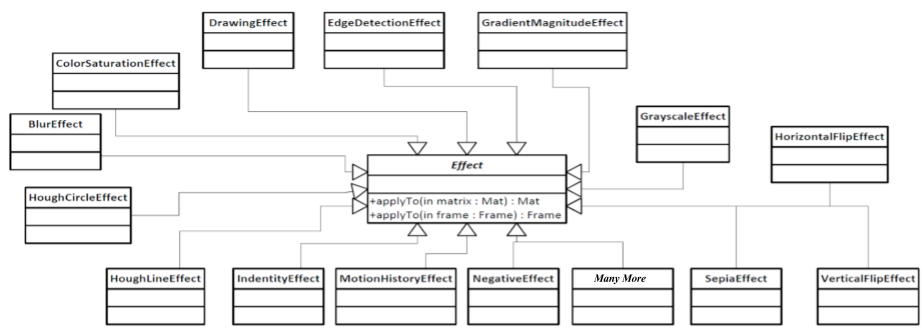
\includegraphics[scale=.2]{Effects.png}
\caption{overview of the Effects.}
\end{figure}
\subsubsection{Definitions}
Below you will find a list of effects we implemented for this project
\begin{itemize}
\item \textit{Blur} \textemdash\space {\tiny Run a Gaussian kernel over an image matrix} 
\item \textit{Circle Detection} \textemdash\space {\tiny  Performs a Hough circle transform}
\item \textit{Color Saturation} \textemdash\space {\tiny Increases the contrast and brightness}
\item \textit{Drawing} \textemdash\space {\tiny Makes a hand drawing like image using image segmentation}
\item \textit{Edge Detection} \textemdash\space {\tiny Takes the gradient of an image using the canny edge detector}
\item \textit{Gradient Magnitude} \textemdash\space {\tiny Takes the gradient of an image, similar to edge detection but reduces the sigma size.}
\item \textit{Gray Scale} \textemdash\space {\tiny reduces the color channels to one}
\item \textit{Horizontal Flip} \textemdash\space {\tiny makes a mirror image}
\item \textit{Line Detection} \textemdash\space {\tiny uses the Hough line transform}
\item \textit{Motion History} \textemdash\space {\tiny keeps track of history and decays older movement} \item \textit{Negative} \textemdash\space {\tiny nots an image}
\item \textit{Sepia} \textemdash\space {\tiny runs a sepia kernel over an image matrix to tint it gold}
\item \textit{Vertical Flip} \textemdash\space {\tiny flips an image across the x axis}
\item \textit{Object Detection} \textemdash\space {\tiny rapid object detection using a boosted cascade of simple features - Car, Cat, Face Features}

\item \textit{Cartoon} \textemdash\space {\tiny Applies a bilateral filter to reduce the color palette of the image and create edge mark from the grayscale image }
\item \textit{Face Detection}\textemdash\space {\tiny  keeping in the tradition of COSMOS we also do face detection}
 \item \textit{Face Landmark Detection} \textemdash\space {\tiny Uses dlib deep learning library to detect face landmark} 
 \item \textit{Mask} \textemdash\space {\tiny Uses dlib deep learning library to detect face landmark and apply a mask on the face}
 
  \item \textit{Face Swap} \textemdash\space {\tiny Uses dlib deep learning library to detect face landmark and swap faces}
\end{itemize}

\begin{figure}[H]
\noindent 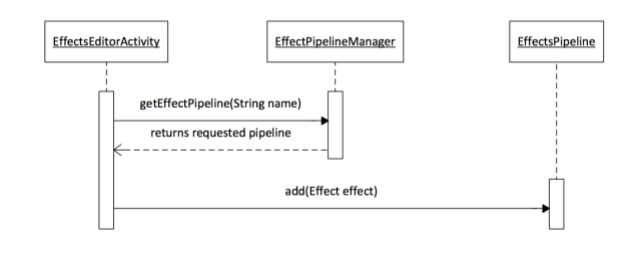
\includegraphics[scale=.3]{EffectsPipline.png}
\caption{Adding an Effect to the pipeline}
\end{figure}

\subsubsection{Example of Effects}
The  effects we chose covered a broad set of Image processing requirements.
\begin{itemize}
\item Image Processing\newline
\begin{tabular}{l | c | r }
\noindent 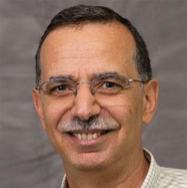
\includegraphics[scale=.3]{OrigImage.png} & 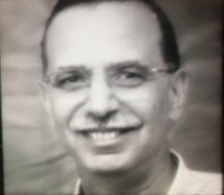
\includegraphics[scale=.3]{grayScale.png} &\noindent 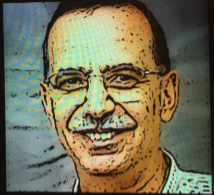
\includegraphics[scale=.3]{CartoonEffect.png} \\
Original & Grayscale & Cartoon \\
\end{tabular}
\item Artificial Intelligence\newline
\begin{tabular}{l | r }
\noindent 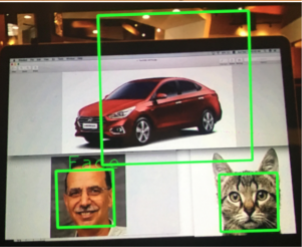
\includegraphics[scale=.2]{ObjectDetection.png} & 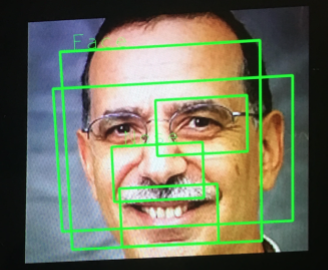
\includegraphics[scale=.2]{FaceFeatureDetection.png} \\ 
Object Detection & Face Feature Detection \\
\end{tabular}
\item Augmented Reality\newline
\begin{tabular}{l | c | r }
\noindent 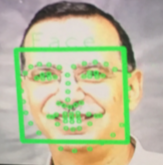
\includegraphics[scale=.3]{FaceLandMarks.png} & 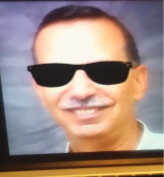
\includegraphics[scale=.3]{MaskEffect.png} &\noindent 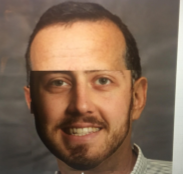
\includegraphics[scale=.3]{FaceSwap.png} \\
{\tiny Face Landmark Detection} & Mask & Face Swap \\
\end{tabular}
\end{itemize}

\section{Implementation}
Our project is a testing framework to measure the practicality of offloading these image processing jobs to a remote server. We do this with an Android application and Java server such that the Java code can be written once and run anywhere. Both of these programs are capable of applying these effects whether or not the choice to offload has been enabled. Our experimentation will be to use a suite of image effects to measure the efficiency of offloading.

\subsection{Client Side}
We built and image manipulation application that  acts as a benchmark suite for common computation problems performed by those in the Computer Vision, Augmented Reality, Artificial Intelligence, and Computer graphics space. We apply multiple filters including some that use neural nets using  OpenCV and Dlib. The Effects themselves were written entirely in Java and thus could be shared with the server side. The Effects classes are inspired by functional programming, they have no global dependencies  and perform their effects without causing any side effects. They take in one input matrix perform and action and return an output matrix. This  makes these effects good candidates to take advantage of pipeline parallelism.

For this project we tried to distinguish ourselves by working with real time data that we get straight from the camera. The effects we have chose make up a range of high, to low computationally complex problem sets. We also implemented a set of  compression optimization's on the client to reduce  the number of bits we send.
    
\subsection{Server Side}
To facilitate the ease of offloading, we use the Apache Avro Interface Description Language, which runs on top of the non-blocking Netty HTTP Web Server.  This IDL is written in a language independent form which is then serialized into JSON and compiled into dependency-free Java.

\begin{figure}[h]
\noindent 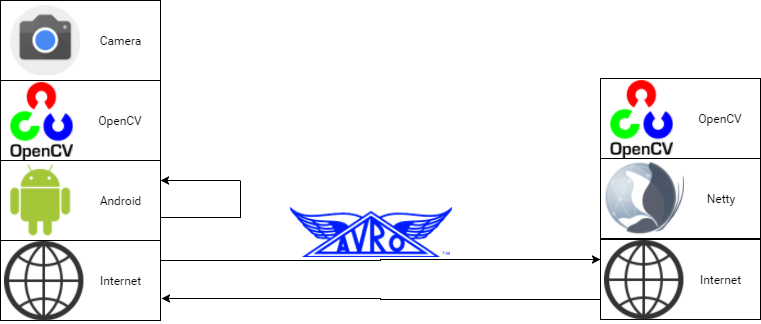
\includegraphics[scale=.3]{ServerOverview.png}
\caption{Overview of the full system pipeline}
\end{figure}


Some benefits of this interface are that we can ship platform-independent code to the client and server which requires no state or previous interaction to complete a task. The compiled Java code is a loose interface which abstracts device dependant implementations. Because each task is modeled as a function call, the profiling tools we use can simply watch the call stack to measure elapsed times, and the Java runtime can take care of any native code discrepancies. 

\subsubsection{Details of Offloading}
 We use Apache Avro to generate the Interface which will be used to implement the offloading framework. An example of an offloadable method, its corresponding AIDL signature and the generated Interface method are given in figure below.
 \begin{figure}[h]
 \begin{tabular}{l  r }
\noindent 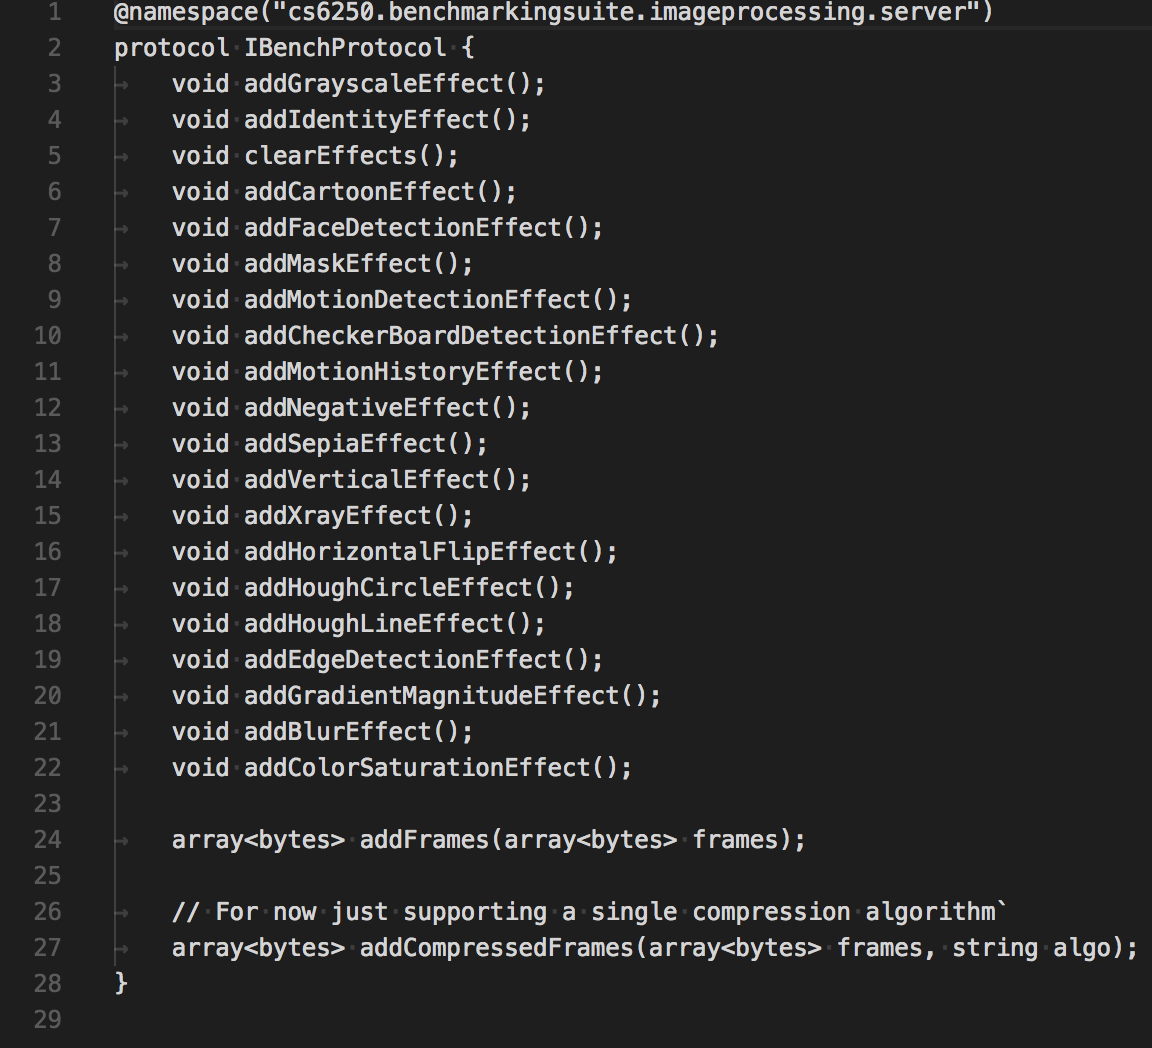
\includegraphics[scale=.2]{AIDLFile.png} & 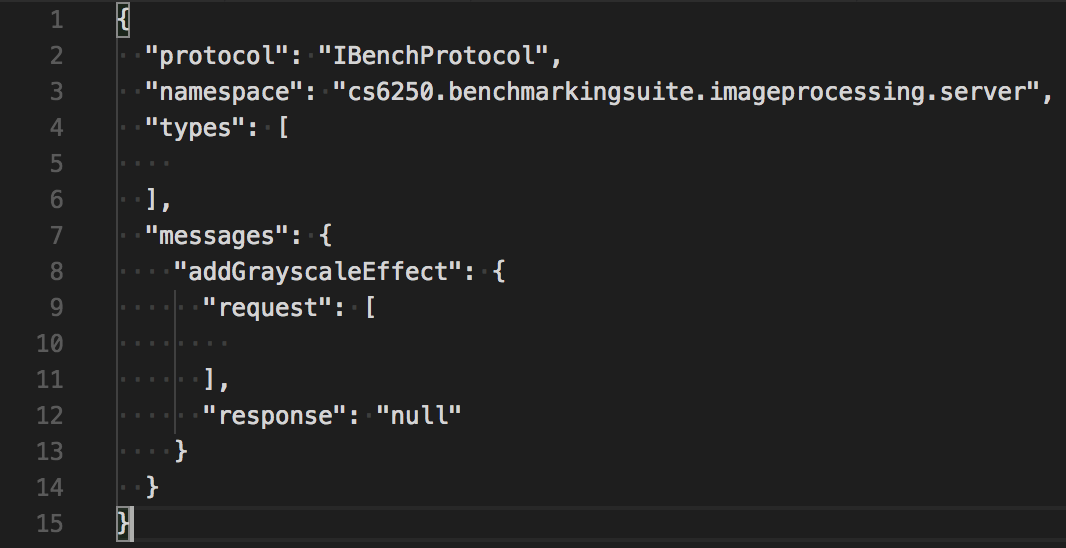
\includegraphics[scale=.2]{AvroGenerated.png} \\ 
\end{tabular}
\caption{AIDL file and the Generate Proxy function's JSON representation}
\end{figure}
To write RPC signatures in AIDL like in the above figure we manually identify which methods can be offloaded. We covered a broad range of algorithms that both should and should not be good at offloading. With profiling we can come up with a minimization subset that we may find suitable for offloading. We need to define some qualitative and quantitative heuristics for offloading. The qualities of methods the literature  suggest are suitable for offloading are:
\begin{itemize}
\item \textit{clean signature} Don't pass around global memory all data passed in or out should be serializable
\item \textit{large execution times} Significant chunk of computation required
\item \textit{System resource independence} Should not require OS or system specific hardware solved with wrappers and interfaces) Examples include camera, storage, and OS specific APIs.
\item \textit{Parallelizable} If a method performs a computation which is much more optimally implemented in the cloud, for example, GPGPU computations, we can choose to offload such a method. For our uses linear algebra and matrices are a very parallelizable problem space.
\item \textit{No native code dependence} The literature encourages the use of  VM only code. This is not something we had the luxury of doing, as both Dlib and OpenCV are native libraries. We get close though by using existing and writing our own JNI wrappers.
\end{itemize}

\section{Profiling}
Everything we have presented so far has been for the sake of answering the one important question of when should we offload? Using Android's Traceview and iPerf we hope to answer this question.

\subsection{Traceview}
We use Android Traceview to help us determine which Effects are good candidates to offload. Traceview is an android tool used for profiling an applications performance and produces execution trace logs with per method execution times that we can comb over with out own scripts. It gives us detailed view of the execution times of a method as well as their call stacks. Using a Traceview profile, we  can build up a heuristic to determine offload candidates.
\subsection{iPerf3}
Traceview above let us know either the time to run on device or the time to run on the server plus communication time. However, this alone is not enough information to determine if we should offload For this we need iPerf3, a bandwidth measurement tool. We ported iPerf3 to android and then began measuring the available bandwidth for our app and the health of our network. With the information provided by iPerf and Traceview we can finally do something smart, like dynamic offloading.

\section{Experimentation}
\subsection{Method}
We evaluated our project across three different simulated mobile networking scenarios:
\begin{itemize}
\item \textbf{WiFi} a connection over enterprise-grade 802.11 wireless access point between our RPC server on one machine and an emulator on another. 
\item \textbf{3G} Here we rate limit the emulators network speeds to that of a 3G modem.
\item \textbf{4G} Here we rate limit the emulators network speed to that of a 4G modem.
\end{itemize}
For a baseline we measured the on-device computation of each image effect defined in the effects section of this paper.Then for each of the scenarios listed above we calculated the performance of each effect when offloaded. We also wanted to experiment with compression optimizations. So we had a test looking for both the fastest and most reduced sized payload. The best algorithm was then run across the full set of effects to evaluate performance.   
Each run had both iPerf as well as Traceview runs. This generated server and client side iPerf files as well as one trace dump file that we evaluated for performance metrics.

To reduce variability among results we all used an x86 QEMU emulated Pixel android phone running Android 8 Oreo.

Next, we decided to run the results on different network link speeds. This is because mobile applications today run applications on both cellular data at 3G or 4G/LTE speeds as well as on WiFi. The experiments were conducted by limiting the emulator network rates to match the real world data rates as closely as possible.

The Traceview data was collected for all effects initially to determine the CPU usage for each effect on device and on server. Next, the iPerf logs were used to determine the network utilization during offloading. So, the idea was to use the data from Traceview and iPerf to determine the CPU and network utilization for different types of effects.

The compression bandwidths vs Time Figures show that the gzip and bzip2 offer the best maintenance of bandwidth when the effect type was held constant across multiple network types.  The two anomalous data entries in the Face Landmark and Face Swap in the Time to Compute graph were likely caused by invocation of the android dynamic loader for the dLib module.

\subsection{Results}

\begin{tikzpicture}
\begin{axis}[
    title={3G Bandwidth vs Time},
    xlabel={Time (ms)},
    ylabel={Bandwidth (Kbps)},
    xmin=0, xmax=10,
    ymin=60000, ymax=160000,
    xtick={0, 1, 2, 3, 4, 5, 6, 7, 8, 9, 10},
    ytick={60000,80000,100000,120000,140000,160000},
    legend pos=north west,
    ymajorgrids=true,
    grid style=dashed,
]
 
\addplot[
    color=blue,
    mark=square,
    ]
    coordinates {
    (0.5, 80725.66667)(1.5,90553.33333)(2.5,102817)(3.5,107616.3333)(4.5,106640)(5.5,103611)(6.5,91741)(7.5,96752.33333)(8.5,96716)(9.5,94534.66667)
    };

\addplot[
    color=red,
    mark=square,
    ]
    coordinates {
    (0.5, 75386)(1.5,91831.66667)(2.5,93129.66667)(3.5,93761.66667)(4.5,73998.33333)(5.5,73513.66667)(6.5,80480)(7.5,95012.66667)(8.5,98362.33333)(9.5,90805.66667)
    };

    
\addplot[
    color=green,
    mark=square,
    ]
    coordinates {
    (0.5, 79591.33333)(1.5,95515)(2.5,90740.33333)(3.5,92860)(4.5,105850.6667)(5.5,101589.6667)(6.5,94291)(7.5,108560)(8.5,92673.33333)(9.5,98276)
    };
    
    
\addplot[
    color=orange,
    mark=square,
    ]
    coordinates {
    (0.5, 69885.33333)(1.5,88093)(2.5,79755.33333)(3.5,73951)(4.5,65401.33333)(5.5,86747.33333)(6.5,78278.66667)(7.5,84618.33333)(8.5,68699.66667)(9.5,78512)
    };
\legend{bzip2,deflate, gzip, lz4}
\end{axis}
\end{tikzpicture}


\begin{tikzpicture}
\begin{axis}[
    title={4G Bandwidth vs Time},
    xlabel={Time (ms)},
    ylabel={Bandwidth (Kbps)},
    xmin=0, xmax=10,
    ymin=60000, ymax=160000,
    xtick={0, 1, 2, 3, 4, 5, 6, 7, 8, 9, 10},
    ytick={60000,80000,100000,120000,140000,160000},
    legend pos=north west,
    ymajorgrids=true,
    grid style=dashed,
]
 
\addplot[
    color=blue,
    mark=square,
    ]
    coordinates {
    (0.5, 86330.33333)(1.5,95152.33333)(2.5,95266)(3.5,102757.3333)(4.5,95865.33333)(5.5,98526)(6.5,102369.6667)(7.5,106024)(8.5,102407.3333)(9.5,105961)
    };

\addplot[
    color=red,
    mark=square,
    ]
    coordinates {
    (0.5, 98840)(1.5,94425.33333)(2.5,99103)(3.5,102878.6667)(4.5,106131)(5.5,104549)(6.5,102072)(7.5,107071.6667)(8.5,107028.6667)(9.5,108234.3333)
    };

    
\addplot[
    color=green,
    mark=square,
    ]
    coordinates {
    (0.5, 82405)(1.5,86961)(2.5,85066.66667)(3.5,97607.66667)(4.5,95608.33333)(5.5,97731)(6.5,99374.66667)(7.5,104361.6667)(8.5,102638.6667)(9.5,103535.6667)
    };
    
    
\addplot[
    color=orange,
    mark=square,
    ]
    coordinates {
    (0.5, 80581.33333)(1.5,97317.33333)(2.5,92321.33333)(3.5,98541.66667)(4.5,102055.3333)(5.5,106154.3333)(6.5,107097.6667)(7.5,106876.3333)(8.5,109861.3333)(9.5,104201.6667)
    };
    
\addplot[
    color=brown,
    mark=square,
    ]
    coordinates {
    (0.5, 69885.33333)(1.5,88093)(2.5,79755.33333)(3.5,73951)(4.5,65401.33333)(5.5,86747.33333)(6.5,78278.66667)(7.5,84618.33333)(8.5,68699.66667)(9.5,78512)
    };
    
\legend{bzip2,deflate, gzip, lz4, snappy}
\end{axis}
\end{tikzpicture}


\begin{tikzpicture}
\begin{axis}[
    title={Wifi Bandwidth vs Time},
    xlabel={Time (ms)},
    ylabel={Bandwidth (Kbps)},
    xmin=0, xmax=10,
    ymin=60000, ymax=280000,
    xtick={0, 1, 2, 3, 4, 5, 6, 7, 8, 9, 10},
    ytick={60000,80000,100000,120000,140000,160000,180000,200000,220000,240000,260000,280000},
    legend pos=north east,
    ymajorgrids=true,
    grid style=dashed,
]
 
\addplot[
    color=blue,
    mark=square,
    ]
    coordinates {
    (0.5, 108563)(1.5,114613)(2.5,119293)(3.5,117644)(4.5,107694)(5.5,135251)(6.5,127710)(7.5,133097)(8.5,124089)(9.5,153424)
    };


\addplot[
    color=red,
    mark=square,
    ]
    coordinates {
    (0.5, 159115)(1.5,194539)(2.5,180269)(3.5,178412)(4.5,178412)(5.5,172817)(6.5,164405)(7.5,157949)(8.5,169723)(9.5,168581)
    };
    
\addplot[
    color=green,
    mark=square,
    ]
    coordinates {
    (0.5, 142845)(1.5,158430)(2.5,162716)(3.5,187823)(4.5,260233)(5.5,169720)(6.5,117297)(7.5,157366)(8.5,146463)(9.5,149585)
    };
    
    
\addplot[
    color=orange,
    mark=square,
    ]
    coordinates {
    (0.5, 160999)(1.5,183593)(2.5,190875)(3.5,179521)(4.5,171146)(5.5,183625)(6.5,191039)(7.5,168891)(8.5,167672)(9.5,159721)
    };
    
\addplot[
    color=brown,
    mark=square,
    ]
    coordinates {
    (0.5, 92210)(1.5,110577)(2.5,102137)(3.5,107930)(4.5,113413)(5.5,112549)(6.5,122540)(7.5,114955)(8.5,121771)(9.5,120368)
    };
    
\legend{bzip2,deflate, gzip, lz4, snappy}
    
\end{axis}
\end{tikzpicture}

\begin{figure*}%* is used because without it the figure does not appear
\begin{center}
\begin{tikzpicture}
\begin{axis}[
    title={iPerf CPU Utilization \% of Device and Server Across Effects},
    ybar,
    enlargelimits=0.15,
    width=15cm,
     height=8cm,
    legend style={at={(0.5,-0.15)},
      anchor=north,legend columns=-1},
    ylabel={CPU Utilization \%},
    xlabel={Effect},
    symbolic x coords={Cartn,Cat,FacFea,FacLm,FacSwp},
    xtick=data,
    nodes near coords,
    nodes near coords align={vertical},
    ]
\addplot coordinates {(Cartn,51) (Cat,57) (FacFea,63) (FacLm,60) (FacSwp,59)};
\addplot coordinates {(Cartn,10) (Cat,10) (FacFea,10) (FacLm,11) (FacSwp,11)};
\legend{Device,Server}
\end{axis}
\end{tikzpicture}
\end{center}
\end{figure*}


\begin{figure*}
\begin{center}
\begin{tikzpicture}
\begin{axis}[
    title={Overall Time to Compute when Offloaded and On-Device Across Effects},
    ybar,
    enlarge y limits={upper=0},
    width=15cm,
     height=10cm,
    legend style={at={(0.5,-0.15)},
      anchor=north,legend columns=-1},
    ylabel={Time to Compute (ms)},
    xlabel={Effect},
    symbolic x coords={FacFea,FacLm,FacSwp,Cat,Cartn,GraSc,MotHis,GradMg,Neg,Sep},
    xtick=data,
    nodes near coords,
    nodes near coords align={vertical},
    ]
    
\addplot+[error bars/.cd,
y dir=both,y explicit]
coordinates {
(FacFea,101) +- (0.0, 35.97)
(FacLm,102) +- (0.0, 31.02)
(FacSwp,94) +- (0.0, 15.16)
(Cat,87) +- (0.0, 16.89)
(Cartn,76) +- (0.0, 11.06)
(GraSc,25) +- (0.0, 1.13) 
(MotHis,19) +- (0.0, 0.39)    
(GradMg,14) +- (0.0, 0.70)
(Neg,11) +- (0.0, 0.27)
(Sep,11) +- (0.0, 0.52)};

\addplot
coordinates {
(FacFea,4208) 
(FacLm,19250) 
(FacSwp,19438) 
(Cat,144)
(Cartn,4440) 
(GraSc,8)  
(MotHis,8)     
(GradMg,13)
(Neg,7)
(Sep,15)};
	 

\legend{Offload,On-Device}

\end{axis}
\end{tikzpicture}
\end{center}
\end{figure*}
\begin{figure}[H]
\noindent 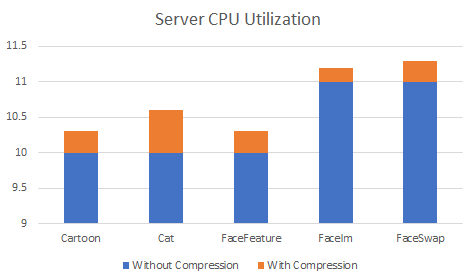
\includegraphics[scale=.5]{Graph1.png}
\caption{CPU Utilization on device.}
\end{figure}
\begin{figure}[H]
\noindent 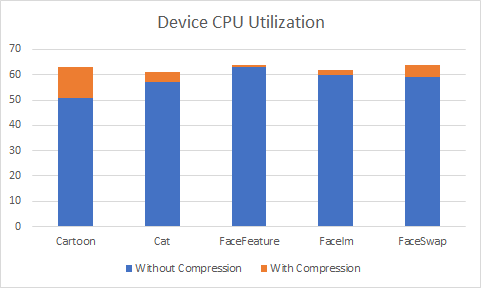
\includegraphics[scale=.5]{Graph2.png}
\caption{CPU Utilization on Server.}
\end{figure}

\section{Future Work}
\subsection{Simplified Dynamic Offloading Decision Engine}
The decision engine we have experimented with but need more data to complete is based on the following:

\begin{itemize}
\item bandwidth to the server
\item computation time on the server
\item computation time locally
\end{itemize}

We need to determine what our communication costs will be for this we will define
the following formula for time to communicate. (Note we multiply by 2 to account for sends and receives.)
\begin{equation}
T_{total\_communication} = 2 * \frac{Size_{image}}{bandwidth}
\end{equation}

We can estimate the amount of time taken to process the image on the server when
offloaded as follows:

\begin{equation}
T_{total\_server} = T_{total\_communication} + T_{computation\_server}
\end{equation}

To determine what are good candidates for offloading we need to 
statically compute the average amount of time required to apply an effect to
an image both on the server ({\it T$_{computation\_server}$}) and on the local
device ({\it T$_{computation\_device}$}). This is where our Traceview Runs come in handy.

If T$_{computation\_server}$ is less than T$_{computation\_device}$ then we have a candidate
for offloading. But as mentioned above in the iPerf section that is not enough data. 
We start with a fuzzed value of 100 ms to represent communication costs at first 
until we can update with a more accurate number representing the current state of the network.
If T$_{total\_server}$ is greater than T$_{comp\_dev}$, it means that it is more
efficient to do the computation locally than offloading. This decision is taken
dynamically. Using the information surmised above we can use the 
following heuristic (equation 3) to determine when to offload.
\begin{equation}
 T_{computation\_device} > T_{total\_server}
\end{equation}

\begin{figure}[H]
\noindent 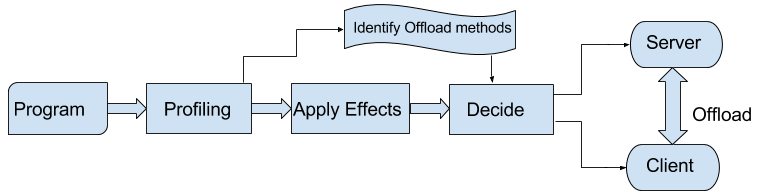
\includegraphics[scale=.3]{DecisionEngine.png}
\caption{The Decision Engine pipeline}
\end{figure}

\subsection{Video Codec Optimizations}
The project can be extended to work with live video streams, to process these video streams on device or on cloud. Video streams carry large amounts of data. Consider a 480p video stream at 30 frames per second with 24 bits per pixel (colored video). It generates data at the rate of 221 Mbps. It is not plausible to support such large data rates on today's internet. Hence compression is crucial. \cite{codec}

Video streams can be broken down into frames where each frame is essentially an image. A video stream can be compressed spatially and temporally. Spatial video compression is when each frame is compressed individually and temporal compression is when frames are compressed in time. Temporal compression exploits the fact that pixels do not change drastically across each frame. \cite{codec}

Spatial compression uses JPEG (Joint Photographic Experts Group) for compressing each frame. JPEG uses DCT (Discrete Cosine Transform) encoding with quantization to achieve compression. Another aspect is using YUV and chroma subsampling. Using chroma subsampling, we can send color data at half the resolution. This is because human eye cannot detect changes in color as sharply as changes in brightness. \cite{codec}

However, in high motion frames,it is more important to send more number of frames than maintaining the resolution of each frame. Hence, a new macroblock encoding technique can be used, "Flat", to reduce the bits needed for each frame. Flat format is:

6 bits - for each color channel quantized by 4 \cite{codec}

DCT and quantization is done to reduce the coefficient values to zero to save bandwidth. However, what is more important is getting the consecutive coefficients to zero so that we can use RLE (Run Length Encoding) to actually reduce the number of bits to be sent. \cite{codec}

For this, we need to focus on the entropy coding. JPEG uses Huffman coder to reduce the number of bits sent for coefficients closer to zero. An artithmetic coder like RANS can aslo be used to save bandwidth. \cite{codec}

\section{Conclusion}
In the paper, we have implemented a testing framework to measure the practicality of offloading image processing jobs to a remote server. The experimental results show that our system enables computation offloading at low cost and high efficiency. We have noticed the best offloading performance in our ML based algorithms like face swap, Even when accounting for the additional performance cost at start up of shared library loading we still see reliable performance improvements.

There are some future directions to extend our testing framework. We need more data to complete bandwidth to the server, computation time on the server and computation time locally for simplified dynamic offloading decision engine. The project can be extended to work with live video streams, to process these video streams on device or on cloud. 

\begin{thebibliography}{2}

\bibitem{cosmos} 
Cong Shi, Karim Habak, Pranesh Pandurangan,Mostafa Ammar, Mayur Naik, Ellen Zegura 
\textit{COSMOS: Computation Offloading as a Service for MobileDevices}. 

\bibitem{clonecloud} 
Byung-Gon Chun, Sunghwan Ihm, Petros Maniatis, Mayur Naik, Ashwin Patti
\textit{CloneCloud: Elastic Execution between Mobile Device and Cloud}. 

\bibitem{wifiBattery}
Ning Ding Daniel Wagner Xiaomeng Chen Abhinav Pathak Y. Charlie Hu Andrew Rice
\textit{Characterizing and Modeling the Impact of Wireless Signal Strength on Smartphone Battery Drain}.

\bibitem{darkSilicon}
Max Menges
\textit{Dark Silicon and its Implications for Future Processor Design}

\bibitem{partitioning}
Jianqiang Li, Luxiang Huang, Yaoming Zhou, Suiqiang He, and Zhong Ming
\textit{Computation Partitioning for Mobile Cloud Computing in a Big Data Environment}

\bibitem{greenDroid}
Nathan Goulding, Jack Sampson, Ganesh Venkatesh, Saturnino Garcia, Joe Auricchio, Jonathan Babb, Michael B. Taylor, and Steven Swanson
\textit{GreenDroid: A Mobile Application Processor for a Future of Dark Silicon}

\bibitem{HoughLineTransform1}
\url{http://docs.opencv.org/doc/tutorials/imgproc/imgtrans/hough_lines/hough_lines.html}

\bibitem{HoughLineTransform2}
\url{http://www.aishack.in/2010/04/hough-transform-in-opencv/}

\bibitem{SobelOperator}
\url{http://docs.opencv.org/doc/tutorials/imgproc/imgtrans/sobel_derivatives/sobel_derivatives.html}

\bibitem{Canny Edge detection}
\url{http://docs.opencv.org/doc/tutorials/imgproc/imgtrans/canny_detector/canny_detector.html}

\bibitem{AndroidRefactor}
Ying Zhang, Gang Huang , Xuanzhe Liu , Wei Zhang, Hong Mei, Shunxiang Yang
\textit{Refactoring Android Java Code for On-Demand Computation Offloading}

\bibitem{codec}
Ben Garney
\textit{https://bengarney.com/2016/06/25/video-conference-part-2-joint-photographic-hell-for-beginners/ Video Conference: Joint Photographic Hell (For Beginners)}


\end{thebibliography}

\end{document}